\documentclass[conference]{IEEEtran}
\usepackage{amsmath}
\usepackage{booktabs}
\usepackage{graphicx}
\usepackage{subcaption}
\usepackage{url}
\usepackage{tikz}

\title{When Does 2\,MiB Page Granularity Still Matter for vAttention?\\
Empirical and Analytical Tail-Waste Characterization Across MHA, GQA, and MLA}

\author{\IEEEauthorblockN{Project Team}
\IEEEauthorblockA{University Course Project}}

\begin{document}
\maketitle

\begin{abstract}
In the context of large language model inference, the 
KV cache stores the key and value activations needed to reuse 
prior attention state during autoregressive decoding, so 
reducing its memory footprint directly improves throughput, 
batch size, and the maximum practical context length. 
vAttention was proposed as an alternative to vLLM's PagedAttention to 
preserve contiguous virtual memory for the KV cache while 
relying on GPU demand paging for on-demand physical allocation. 
This let the system to reuse unmodified high-performance kernels, 
including FlashAttention, instead of requiring paging-aware 
attention kernels and explicit block-table management in the 
serving stack. The vAttention paper reported up to $1.97\times$ 
faster token generation than vLLM and up to $3.92\times$ and 
$1.45\times$ faster prompt processing than the PagedAttention 
variants of FlashAttention and FlashInfer. However, under 
the stock NVIDIA driver path, this design is constrained 
by a 2\,MiB page granularity, which can still create non-trivial 
tail waste. The vAttention project mitigated this waste by implementing 
a custom open source NVIDIA driver.
This project asks whether the custom vAttention driver path 
is still necessary once context lengths become large. 
We characterize tail-waste fragmentation under a fixed 2\,MiB 
page size for three attention families: multi-head attention (MHA), 
grouped-query attention (GQA), and multi-head latent attention (MLA). 
Our evaluation covers Qwen-14B (MHA), Mistral-Nemo-12B (GQA), 
DeepSeek-V2-Lite (MLA), and a novel synthetic Mistral MLA 
implementation that we added to the vAttention codebase 
to enable a controlled GQA versus MLA comparison on the same backbone. 
The answer to the primary question is conditional. 
Some models can reach context ranges where 2\,MiB tail 
waste becomes insignificant, but architectural improvements, like GQA and MLA,
also change the fragmentation curve and can push that crossover 
point far to the right. This ambiguity motivates our second 
contribution: an analytical model that predicts tail-waste fragmentation 
from model parameters and context length. The measured runs and 
side-by-side analytical comparisons show that these predictions 
closely match observed sawtooth behavior, giving system implementors a 
practical way to decide whether deploying the custom vAttention 
driver is worthwhile for their target context range and model architecture.
\end{abstract}

\section{Introduction and Background}
Large language model serving systems increasingly rely on paged KV-cache 
management to scale long-context inference. Paged designs reduce copying 
and simplify memory reuse, but they introduce \emph{tail waste}: 
the final mapped page of a request is rarely perfectly full. 
vAttention addresses this problem with a custom driver path that can 
reduce the page size from 2\,MiB to 64\,KiB. The practical deployment 
question is whether that additional systems complexity is still 
justified as context windows get longer.

Our primary research question is:
\begin{quote}
\emph{Do we still need the vAttention custom driver that reduces page size from 2\,MiB to 64\,KiB, even at long context lengths?}
\end{quote}

We began from the intuition in our proposal that 2\,MiB pages 
might be ``good enough'' for sufficiently long contexts, 
especially for dense architectures such as MHA. That intuition 
was only partly correct. Once we compared multiple attention 
architectures, the answer became more nuanced. Efficient attention 
layouts reduce bytes per token, therefore under a fixed 2\,MiB page
size the number of tokens that fit into each page increases. As a result,
the tail-waste percentage decreases more slowly as context grows, and the
context length required to push fragmentation below a threshold such as
$5\%$ can become much larger than we originally expected.

This led to our second research question:
\begin{quote}
\emph{How can a user know in advance when 2\,MiB pages will cause significant tail waste for a given model and target context range?}
\end{quote}

The contribution of this project is therefore twofold. 
First, we built an experimental pipeline that characterizes tail waste 
across architectures. Second, we derived and validated analytical 
formulas that predict the fragmentation curve from model parameters 
and context length. A further novel systems contribution is that we 
added an MLA implementation path to the vAttention codebase 
used in this project, including a synthetic Mistral MLA path. 
That extension made the controlled GQA versus MLA comparison possible.

\section{Design and Implementation}
Our implementation extends the vattention repository in three main directions.

\subsection{Measurement pipeline}
We added an end-to-end experimental pipeline that starts a model server, 
sends one request at a time with exact prompt token counts, records 
per-request metrics, and generates plots from the resulting CSVs. 
The pipeline writes host-visible outputs under \texttt{server-output/} 
and derived figures under \texttt{server\_plots/}. The resulting 
measurements are based on a single active request with \texttt{max\_tokens=1}, 
which isolates allocator tail waste from unrelated batch interactions.

\subsection{MLA support and synthetic Mistral MLA}
The repository state we started from only supported dense 
attention layouts such as MHA and GQA. During this project we 
added MLA support to the vAttention codebase from scratch, including 
the cache-layout abstractions, runtime integration, model scaffolding, 
and DeepSeek-V2-Lite serving path needed to exercise a real MLA model. 
We then extended that work with \texttt{MistralMLAForCausalLM} and 
the supporting loader and configuration logic necessary to run a 
synthetic MLA version of Mistral-Nemo-12B. That second step enabled 
a controlled backbone-matched GQA versus MLA comparison, while 
the broader MLA implementation itself is one of the project's 
primary novel systems contributions.

\subsection{Analytical tail-waste model}
The important distinction from our original proposal is that 
the runtime metric is a \emph{tail-slack percentage in mapped token capacity}, 
not a fixed-byte-waste ratio across the whole cache. Let $C$ be 
context length in tokens, let $T$ be the allocator's number of cached 
tokens per 2\,MiB page, and let $B(C)=\lceil C/T\rceil$ be the number of
blocks (pages) allocated for that request. Figure~\ref{fig:fragmentation-intuition}
shows the resulting mapped capacity, used capacity, and tail slack. The exact
fragmentation law used by the runtime is
\begin{equation}
F_{\text{exact}}(C)=100\cdot\frac{\lceil C/T \rceil T - C}{\lceil C/T \rceil T}.
\end{equation}
This produces the empirical sawtooth shape directly. For a smooth upper 
envelope, we use
\begin{equation}
F_{\text{worst}}(C)\approx 100\cdot\frac{T}{C+T}.
\end{equation}
We also retain the average approximation from the original intuition 
that the final page is half full on average:
\begin{equation}
F_{\text{avg}}(C)\approx 100\cdot\frac{T/2}{C+T/2}.
\end{equation}
In the paper figures, we use $F_{\text{worst}}$ as the main 
overlay because it cleanly predicts the vertical scale of the 
measured peaks, while $F_{\text{exact}}$ is used for side-by-side validation.

\begin{figure}[t]
\centering
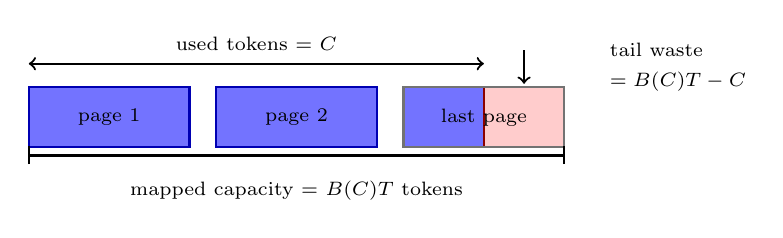
\begin{tikzpicture}[x=0.85cm,y=0.85cm]
  \draw[fill=blue!55,draw=blue!70!black,thick] (0,0) rectangle (2.4,0.9);
  \draw[fill=blue!55,draw=blue!70!black,thick] (2.8,0) rectangle (5.2,0.9);
  \draw[fill=blue!55,draw=blue!70!black,thick] (5.6,0) rectangle (6.8,0.9);
  \draw[fill=red!20,draw=red!55!black,thick] (6.8,0) rectangle (8.0,0.9);
  \draw[draw=black!55,thick] (5.6,0) rectangle (8.0,0.9);

  \node at (1.2,0.45) {\scriptsize page 1};
  \node at (4.0,0.45) {\scriptsize page 2};
  \node at (6.8,0.45) {\scriptsize last page};

  \draw[thick] (0,-0.12) -- (8.0,-0.12);
  \draw[thick] (0,-0.25) -- (0,0.02);
  \draw[thick] (8.0,-0.25) -- (8.0,0.02);
  \node[align=center] at (4.0,-0.65) {\scriptsize mapped capacity = $B(C)T$ tokens};

  \draw[<->,thick] (0,1.25) -- (6.8,1.25);
  \node at (3.4,1.55) {\scriptsize used tokens = $C$};

  \draw[->,thick] (7.4,1.45) -- (7.4,0.95);
  \node[align=left] at (9.7,1.2) {\scriptsize tail waste\\[-1pt]\scriptsize $= B(C)T - C$};
\end{tikzpicture}
\caption{Tail waste under paged KV allocation. A request with context length $C$
maps $B(C)=\lceil C/T\rceil$ pages, each holding $T$ tokens, so the unused
capacity in the final mapped page is $B(C)T-C$.}
\label{fig:fragmentation-intuition}
\end{figure}

The architecture-dependent quantity is $T$:
\begin{equation}
T=\left\lfloor\frac{P}{S_{\text{page-token}}}\right\rfloor,
\end{equation}
where $P=2{,}097{,}152$ bytes is the physical page 
size and $S_{\text{page-token}}$ is the per-token page-buffer footprint.
The terms in $S_{\text{page-token}}$ are not fitted constants. They come
directly from the trained model configuration and therefore from the model
architecture itself. In other words, our analytical predictor uses
architectural parameters already exposed by the model, rather than
reverse-engineering them from the measurements.

For dense KV layouts (MHA/GQA/MQA),
\begin{equation}
T_{\text{dense}}=\left\lfloor\frac{P}{H_{\text{kv,loc}}Db}\right\rfloor,
\end{equation}
where $H_{\text{kv,loc}}$ is the local KV-head count on one tensor-parallel
worker, $D$ is the per-head hidden dimension, and $b$ is the number of bytes
per stored element, e.g., $b=2$ for FP16 or BF16 KV storage. In MHA,
$H_{\text{kv,loc}}$ equals the local attention-head count because every head
has its own key and value vectors. In GQA, multiple query heads share the
same KV heads, so $H_{\text{kv,loc}}$ is smaller, which changes the number of
tokens that fit in a page. For MLA,
\begin{equation}
T_{\text{MLA}}=\left\lfloor\frac{P}{(r_{\text{kv}}+d_{\text{rope}})b}\right\rfloor.
\end{equation}
Here $r_{\text{kv}}$ is the KV latent rank and $d_{\text{rope}}$ is the
dimensionality of the RoPE-encoded key component retained by the MLA cache.
These are also architectural parameters fixed by the trained model design and
reported in the model configuration.
The formulas explain why our original MHA-only proposal was incomplete: the percentage fragmentation curve is controlled by tokens per page, not by total cache bytes per token alone. GQA lowers the local KV-head count and therefore increases $T$ relative to MHA, while MLA replaces dense K/V storage with a latent KV rank and RoPE slice, making $T$ depend on $(r_{\text{kv}}+d_{\text{rope}})$.

We define $5\%$ wasted memory as \emph{insignificant waste}. This threshold is intentionally arbitrary and workload dependent, but it provides a concrete decision boundary. Under the worst-case envelope, the threshold occurs when
\begin{equation}
F_{\text{worst}}(C)\le 5 \iff C\ge 19T.
\end{equation}

\section{Evaluation and Results}
We measured three architectural families under a fixed 2\,MiB page size:
\begin{itemize}
\item Qwen-14B as MHA,
\item Mistral-Nemo-12B as GQA,
\item DeepSeek-V2-Lite as real MLA,
\item synthetic Mistral-Nemo-12B MLA for a backbone-matched GQA versus MLA comparison.
\end{itemize}

The measured tokens per page were:
\begin{itemize}
\item Qwen-14B (MHA): $T=819$
\item Mistral-Nemo-12B (GQA): $T=4096$
\item DeepSeek-V2-Lite (MLA): $T=1820$
\item Mistral-Nemo-12B synthetic MLA: $T=5461$
\end{itemize}

\begin{figure}[t]
\centering
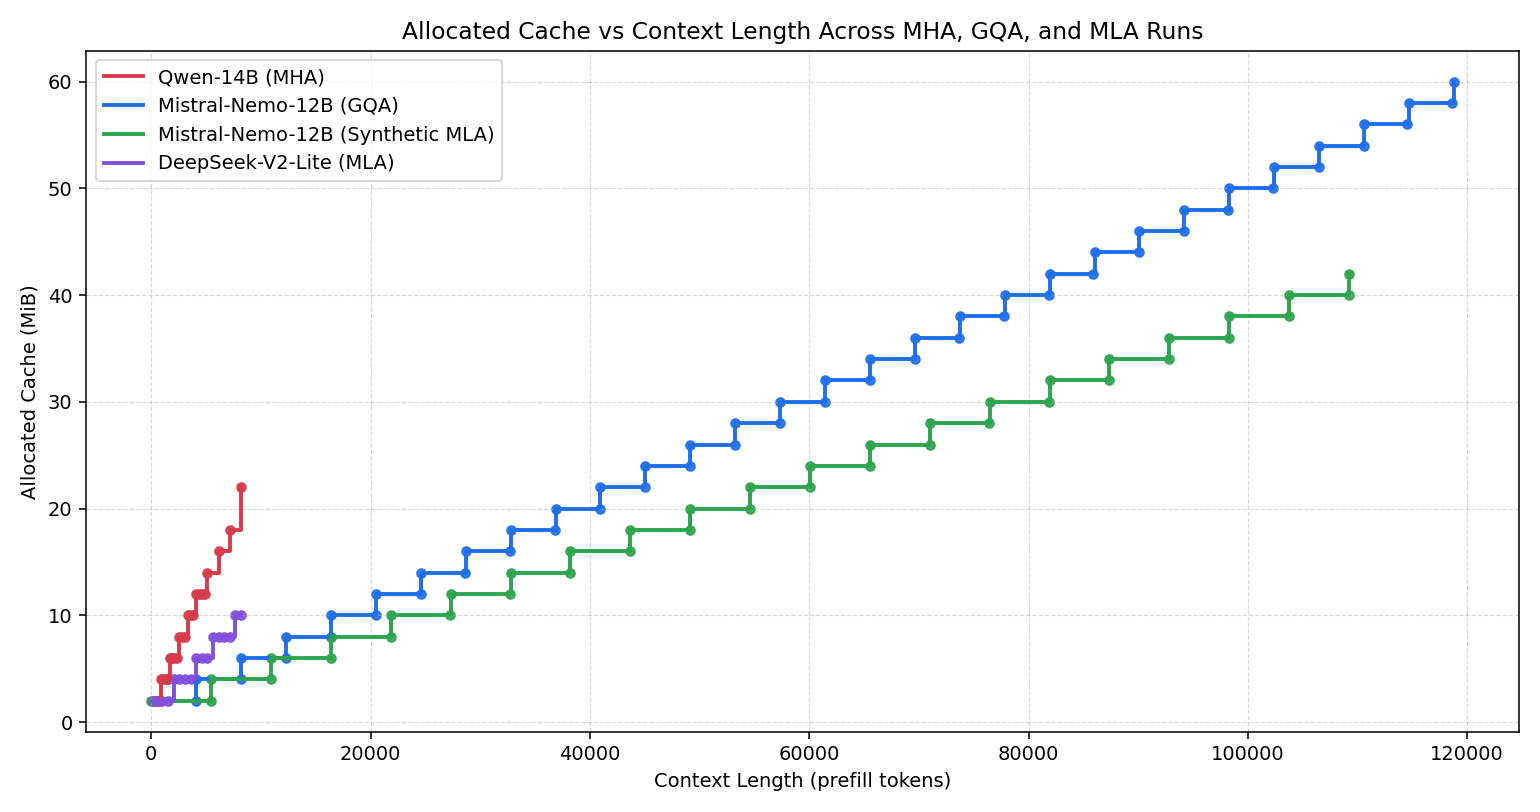
\includegraphics[width=\columnwidth]{../server_plots/comparisons/four-models/cache_bytes_vs_context.png}
\caption{Allocated cache versus context length across the four measured runs. MHA and DeepSeek grow faster in allocated cache than the two Mistral variants, while the synthetic MLA conversion yields the smallest long-context growth among the Mistral pair.}
\label{fig:cache-growth}
\end{figure}

Figure~\ref{fig:cache-growth} answers the first part of the architectural comparison. The four-model cache-growth plot shows that the models do not all scale in the same way. In particular, the Mistral variants are more favorable than Qwen-14B and DeepSeek-V2-Lite in allocated cache growth over the ranges we measured. However, that alone is not enough to answer the driver question, because the relevant metric for the driver is \emph{tail waste percentage}, not just total allocated bytes.

\begin{figure*}[t]
\centering
\begin{subfigure}[t]{0.49\textwidth}
\centering
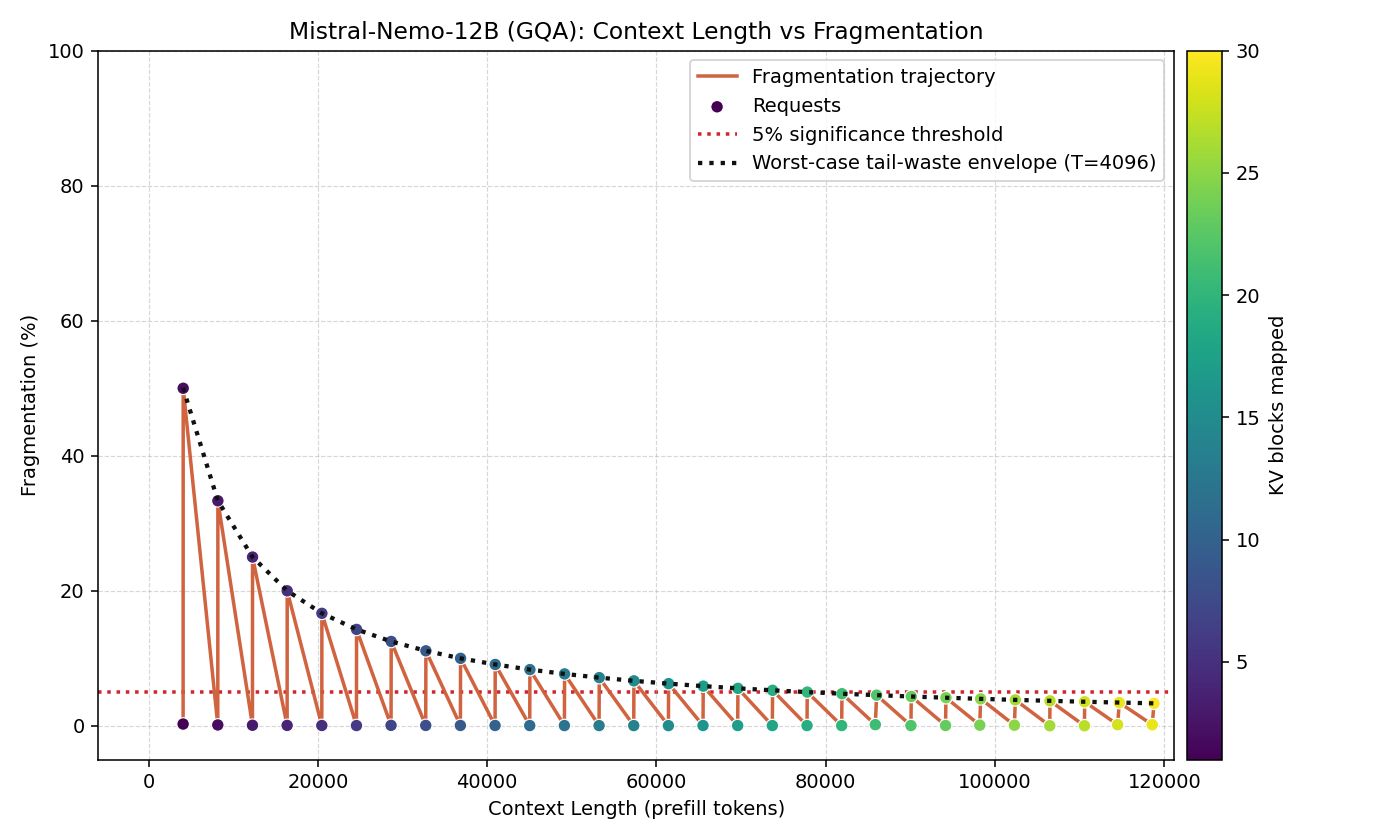
\includegraphics[width=\textwidth]{../server_plots/mistral-nemo-12b/context_vs_fragmentation.png}
\caption{Measured Mistral-Nemo-12B GQA fragmentation with a worst-case analytical envelope.}
\end{subfigure}
\hfill
\begin{subfigure}[t]{0.49\textwidth}
\centering
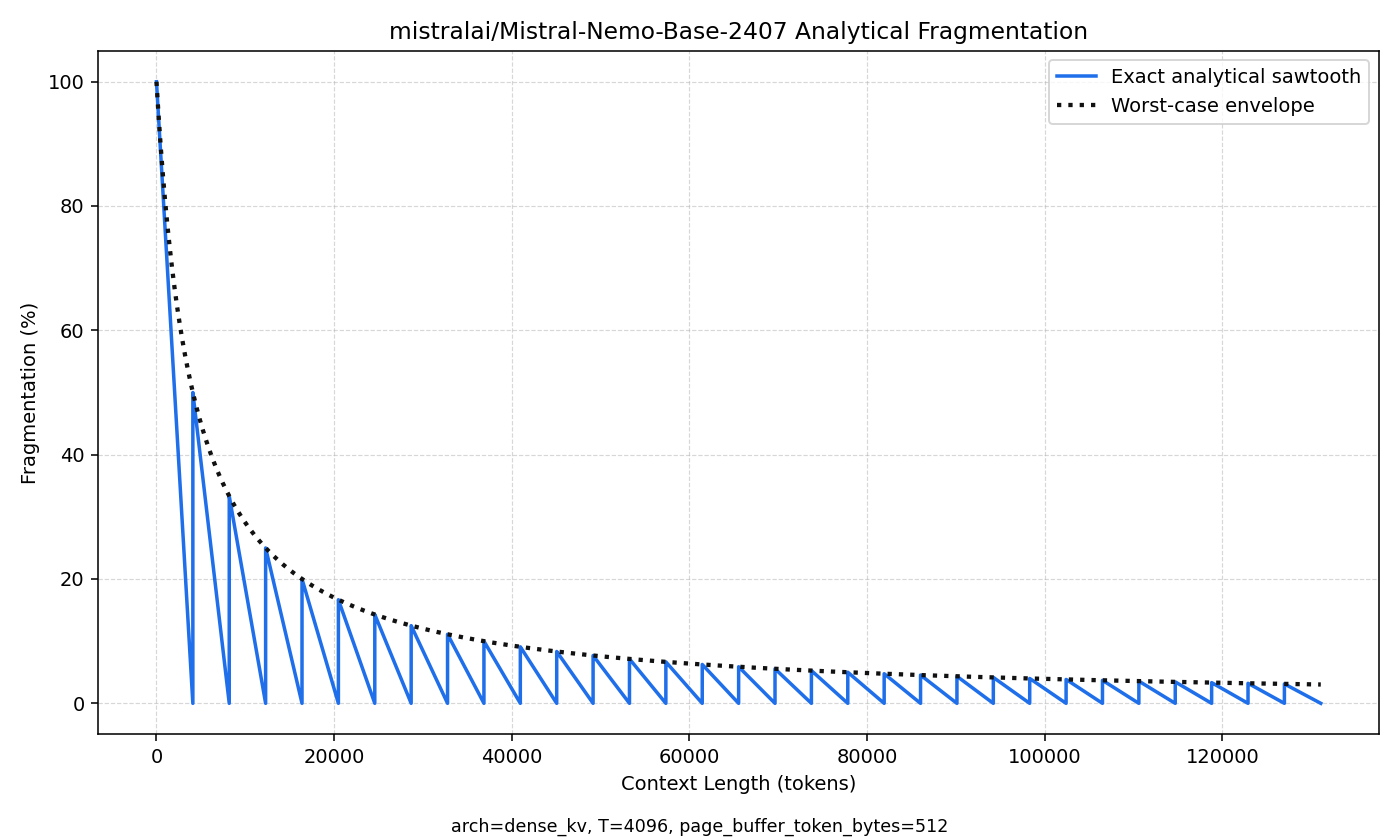
\includegraphics[width=\textwidth]{../server_plots/mistral-nemo-12b/analytical_fragmentation.png}
\caption{Exact analytical sawtooth for the same geometry.}
\end{subfigure}
\caption{Side-by-side empirical and analytical views for Mistral-Nemo-12B. The analytical model predicts the measured tail-waste behavior closely, which supports using model parameters to estimate when 2\,MiB pages become acceptable.}
\label{fig:mistral-analytical}
\end{figure*}

Figure~\ref{fig:mistral-analytical} addresses the second research question. The empirical and analytical curves match closely. The exact analytical prediction error was effectively zero for the short Qwen and DeepSeek runs and remained small for the long Mistral runs: the mean absolute error was approximately $0.06$ percentage points for Mistral GQA and $0.12$ percentage points for synthetic Mistral MLA. That is sufficiently accurate for deployment-oriented decision support.

Using the worst-case threshold $C_{5\%}=19T$, we obtain the following breakpoints:
\begin{center}
\begin{tabular}{lcc}
\toprule
Model & $T$ & $C_{5\%}$ (tokens) \\
\midrule
Qwen-14B (MHA) & 819 & 15{,}561 \\
DeepSeek-V2-Lite (MLA) & 1820 & 34{,}580 \\
Mistral-Nemo-12B (GQA) & 4096 & 77{,}824 \\
Mistral synthetic MLA & 5461 & 103{,}759 \\
\bottomrule
\end{tabular}
\end{center}

These thresholds explain the paper's central conclusion. If a provider offers a very long maximum context, then even 2\,MiB pages may eventually become acceptable. For example, DeepSeek-V2-Lite advertises a much larger model context than the 32\,k cap used in our measured server run, and its analytical threshold occurs around 34.6\,k tokens. In that regime, 2\,MiB tail waste can plausibly become insignificant. But the opposite trend also appears: as attention becomes more memory efficient, each 2\,MiB page holds more tokens, and the $5\%$ threshold shifts farther right. The synthetic Mistral MLA experiment makes this especially clear. Although MLA reduces total memory footprint, it pushes the worst-case insignificance threshold to roughly 103.8\,k tokens, very close to the end of the long-context range we were able to reach experimentally.

Therefore the answer to the primary research question is \emph{it depends}. A user can sometimes get away with the stock 2\,MiB granularity, but the decision depends on architecture and target context range. The best-case scenario for memory efficiency is still the combination of a small page size and an efficient attention layout. Efficient attention does not remove the value of smaller pages; in some cases it increases that value by delaying the point at which tail waste becomes negligible.

\section{Conclusion}
This project set out to determine whether the vAttention custom small-page driver is still necessary at long context lengths. Our experimental answer is conditional rather than absolute. For some models, such as DeepSeek-V2-Lite, long contexts can make 2\,MiB tail waste effectively insignificant. For others, especially when memory-efficient attention increases the number of tokens packed into each page, significant waste can persist deep into the usable context range. The controlled Mistral GQA versus synthetic Mistral MLA comparison demonstrates this complication clearly.

The more useful outcome of the project is not a one-size-fits-all rule, but a predictive method. We showed that tail waste can be predicted from model parameters and context length with high accuracy. That lets users estimate average or worst-case fragmentation over their intended operating range and decide whether the operational overhead of installing custom open-source NVIDIA drivers is justified for their workload.

In addition to answering the research questions, we contributed new implementation capability to the repository by adding MLA support and a synthetic Mistral MLA path, which enabled a novel experimental comparison that was not previously available in this codebase.

\begin{thebibliography}{9}

\bibitem{vattentionrepo}
Microsoft, ``vAttention repository,'' GitHub repository used and extended in this project.

\bibitem{pagedattention}
W. Kwon et al., ``Efficient Memory Management for Large Language Model Serving with PagedAttention,'' in \emph{Proceedings of SOSP}, 2023.

\bibitem{deepseekv2}
DeepSeek-AI et al., ``DeepSeek-V2: A Strong, Economical, and Efficient Mixture-of-Experts Language Model,'' 2024.

\bibitem{mistralnemo}
Mistral AI, ``Mistral-Nemo-Base-2407,'' model release and documentation, 2024.

\bibitem{qwen}
Qwen Team, ``Qwen-14B,'' model release and documentation, 2023.

\end{thebibliography}

\end{document}
